\chapter{Extinction events (I)}

Five major mass extinctions have been recognized.
The most well-documented of which is the Cretaceous--Paleogene (KPB) mass extinction, which happened about 65Ma \cite[p.456]{biomain}.
\footnote{Ma here means Mega (million) years ago}
Shortly following the KPB mass extinction is the Paleocene--Eocene Thermal Maximum (PETM), which is an event marked by a rapid temperature increase, resulting to global climate change that happened approximately 56Ma \cite{Keller2018}.
This chapter will focus on the two events and how they are linked to the current climate crisis and ``mass extinction''.

\section{Effects of KPB and PETM on general global biodversity}
\subsection{Cretaceous--Paleogene Boundary (KPB) mass extinction}
Though the KPB mass extinction was not the most severe mass extinction known, it is the most documented and thus most famous mass extinction event.
\footnote{Numerous films and documentaries focus on the depiction and extinction of dinosaurs.}
A prevailing hypothesis for the mass extinction was that it was triggered when a meteor fell into the Chicxulub crater in Mexico \cite[p.456]{Keller2018, biomain}.
This caused debris to accumulate in the atmosphere and reduced the average amount of solar energy influx to the Earth, decreasing the amount of light and heat.
Since sunlight is vital for photosynthesis of terrestrial plants, which act as primary sources of food, the deficiency of it will result to poorly functioning ecosystems.
There are other hypotheses regarding the KPB extinction event.
These include an eruption of a volcano (Deccan volcano) \cite{Keller2018}.

\citeA{Keller2018} have pointed out criteria for the transition between the Cretaceous and the Paleogene periods.
First is the mass extinction of planktic foraminefera, which was observed from fossils.
Another criterion is the sudden increase of iridium (Ir) in the transition phase.
This is known as the Ir anomaly.
The proponents have argued against the meteor impact theory using the two criteria above by stating that the impact theory dismisses them.
The meteor impact theory, though was formulated based on the observation of the Ir anomaly, ignored the fact that Ir can accumulate in ``redox boundaries in clay layers'' and that volcanic eruptions from the deep mantle can spew out Ir \cite{Keller2018}.
The proponents have also shown evidence of the other criterion using fossil images and comparison, giving validity\footnotemark\ to the Deccan volcano hypothesis.
\footnotetext{My opinion given the evidence.}
They have also suggested that the Chicxulub impact happened prior to the mass extinction crisis, and was not the cause of mass extinction.

Though non-avian dinosaurs got extinct, they were not the only ones to do so \cite[p.456]{biomain}.
Other groups include marine and flying reptiles and ammonites (a type of mollusk).
The biodiversity of angiosperms, birds, and planktons were severely decreased.
However, the biodiversity of turtles, crocodiles, and amphibians were estimated to have remained the same.
The same pattern was also observed in other mass extinctions, which led scientists to believe that mass extinctions do not need to affect all groups of organisms equally \cite[p.456]{biomain}.
Figure \ref{fig:ext} below shows the five major mass extinction events.
\footnote{Image lifted from \cite[p.456]{biomain}.}

\begin{figure}
    \centering
    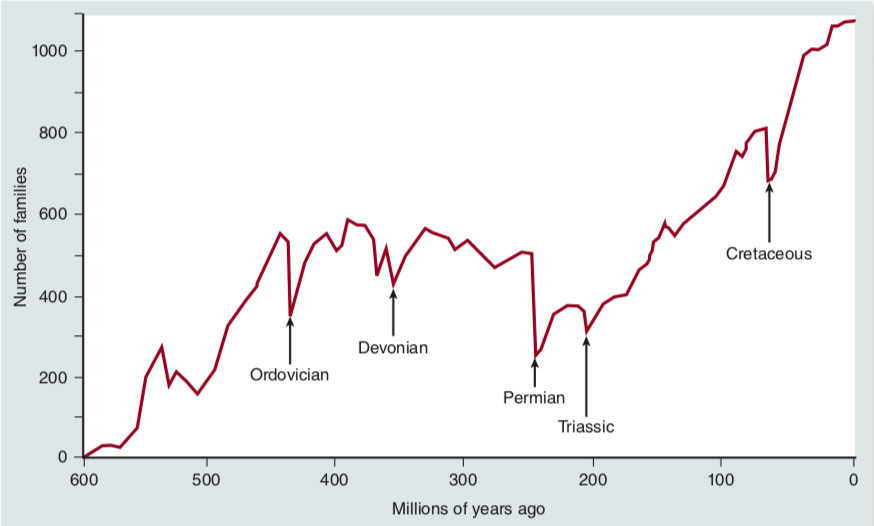
\includegraphics[scale=0.3]{ext}
    \caption{Number of familes with respect to number of years ago. Image shows five major extinction events pointed to by arrows.}
    \label{fig:ext}
\end{figure}

As a consequence of this, previously dominating groups may perish, thus changing the direction of evolution.
This can be related to bifurcation models in complex systems analysis.
\footnote{Introduced in Chapter 1 on complexity}
Non-dominant groups may dominate depending on the conditions following the mass extinction.

\subsection{Paleocene--Eocene Thermal Maximum (PETM)}
The Paleocene--Eocene boundary (PEB) was remarked by the following criteria:

\begin{enumerate}
    \item Disappearance of some benthic foraminefera
    \item Occurrence of some planktic foraminefera
    \item Diversity of \textit{Apectodinium}
\end{enumerate}

A high carbon footprint was found in the atmosphere and oceans possibly coming from volcanic eruptions through methane \cite{Keller2018}, a greenhouse gas.
It was also marked by a global temperature increase of $5-9 ^{\circ}C$ over a course of 30,000 years and ocean acidification.
The high amount of greenhouse gases in the atmosphere may have been responsible for the global temperature increase.
From closer inspection of Figure~\ref{fig:ext}, it can be seen that there is a steep increase in diversity about 10My after the KPB mass extinction.
Fossil records also agree that mammalian migration and diversification happened after the PETM.

\section{Implications in the Anthropocene ``mass extinction''}
From the two events above, \citeA{Keller2018} summarized that rapid increase in global average temperature can cause two things: mass extinction or pseudoextinction.
In both cases there were still extinction events but pseudoextinction in the Eocene period brought diversity.
One of the differences between the Anthropocene mass extinction and the KPB mass extinction is that human niche occupation and economics play vital roles in aggravating the effects of climate change.
Another crucial difference is that humans are aware that they are an agent responsible for the rapid increase in greenhouse gas flux in the atmosphere.
Humans are also able to develop solutions that can alleviate effects and slow down climate change.
